\chapter{Contagens aproximadas}
\label{chap:morris}


Na década de 1970, Robert Morris ~\citep{morris:78} estudou o problema de contar rapidamente \textit{trigramas} cujas 
frequências podiam chegar até 130 mil. Esses eventos eram trios de caracteres que ocorriam em textos.

O objetivo, então, era utilizar as contagens de trigramas na implementação de corretores ortográficos estátisticos 
~\citep{morris:lorinda:75} para editores de textos ~\citep{mcmahon:cherry:morris:78} que acompanhariam as distribuições 
do sistema operacional Unix dos laboratórios da Bell ~\citep{lumbroso:2018}. Contagens similares têm aplicação no 
projeto de compressores de textos estatísticos ~\citep{text:compression:1990}.

Na época, Morris utilizava um computador PDP11 da DEC com memória de 8 bits para realizar as contagens. Com 8 bits, 
somos capazes de representar ou \textit{contar} de 0 até 255. Em geral, uma memória de $n$ bits pode armazenar números 
inteiros entre 0 e $2^{n} - 1$.

Devido à limitação de espaço e ao desejo de eficiência, Morris projetou um algoritmo para realizar estimativas ou 
\textit{contagens aproximadas}, uma vez que, não era possível manter as frequências \textit{exatas} dos trigramas. Com 
seu algoritmo, Morris trouxe aleatorização e probabilidade para o centro da discussão. E para tornarmos essa discussão 
mais precisa, consideraremos o problema de determinar o número de elementos de um dado \textbf{conjunto}~$\Mbb$. 

\begin{quote}
  \textbf{Problema} \proc{ContagemAproximada($\Mbb$)}: dado um conjunto $\Mbb~=~\{ e_1, e_2, \dots, e_n \}$, encontrar 
  estimador $\hat{n}$ para o número $n$ de elementos em $\Mbb$.  
\end{quote}

Quando $\Mbb$ é conhecido de antemão, teremos um problema que é dito \textbf{estático} ou \textit{\textbf{offline}}. 
Já em problemas \textbf{dinâmicos} ou \textit{\textbf{online}}, receberemos uma sequência de operações sobre~$\Mbb$ que 
não são previamente conhecidas e devem ser realizadas uma após a outra. Entre essas operações, existirão as 
\textbf{consultas} (\textit{queries}) que podem ser, por exemplo, encontrar o número de elementos em~$\Mbb$. Teremos, 
também, as \textbf{atualizações} (\textit{updates}) que nesse capítulo, serão modificações de~$\Mbb$ somente por meio de 
inserções de elementos.

Nesse sentido, o problema estudado por Morris pode ser considerado \textbf{incremental} (não há remoções de elementos), 
e dessa forma, o conjunto $\Mbb$ pode ser visto como sendo um \textbf{fluxo} $x_1, x_2, \dots, x_t, \dots$ de elementos, 
e as consultas seriam ``Quantos elementos o conjunto $\Mbb$ possui \textbf{neste instante}~$?$`` ou 
``Quantos elementos já passaram por este fluxo``.

No entanto, estudaremos detalhadamente nesse texto, as versões estatícas dos problemas apresentados, uma vez que, as 
análises dos algoritmos que resolvem esses problemas se baseiam nessas versões. E veremos que obter a versão 
\textit{online} a partir da \textit{offline} é uma tarefa simples, e assim, as aplicações e simulações desses algoritmos 
serão baseadas em versões dinâmicas.

\section{Algoritmo de Morris}

Para armazenarmos \textit{exatamente} um valor entre $0$ e $n$, são necessários registradores com~$\Omega(\lg n)$ bits. 
Então, para que seja possível contar o número de elementos em um conjunto~$\Mbb$ com até $n$ elementos usando menos 
bits, devemos abandonar a \textit{exatidão} da contagem e buscar alternativas aceitáveis.

Morris sugeriu utilizar um contador $X$ para armazenar o valor de $\lg n$ ao invés de $n$. Neste caso, o estimador 
\textit{aproximado} $\hat{n}$ de $n$ seria~$2^{X} - 1$. Este ``-1`` na expressão faz com que essa aproximação se ajuste 
à situação em que $\Mbb = \emptyset$. E um contador como este pode ser armazenado em $O(\lg X) = O(\lg \lg n)$ bits.

A política de incremento de $X$ passa a ser a questão central do algoritmo. Morris propôs uma estratégia simples para 
realizar esse acréscimo: a cada novo elemento examinado de~$\Mbb$, o contador $X$ seria incrementado com probabilidade~ 
$2^{-X}$.

Essa estratégia pode ser vista no Algoritmo $\proc{Morris}$ cuja implementação é baseada em uma ideia da seção 
\textit{Algorithm} do artigo ~\citetitle*{ApproximateCountingAlgorithm}~\citep{ApproximateCountingAlgorithm}.Essa versão 
expressa a condição de incremento do contador como um experimento de lançamento de moedas. Sempre que um novo elemento 
do conjunto $\Mbb$ é examinado, o lançamento de $X$ moedas é simulado. O contador é incrementado somente quando os 
resultados de todos os lançamentos forem cara. E a probabilidade deste evento ocorrer é~$2^{-X}$.

O Algoritmo $\proc{Morris}$ a seguir recebe um conjunto~$\Mbb = \{ e_1, e_2, \dots, e_n \}$ e devolve um estimador~
$\hat{n}$ para $n$. Este estimador é da forma $2^{X} - 1$ em que $X$ é um número inteiro não negativo, e veremos mais 
adiante que o seu valor esperado é $n$, ou seja, $\Ebb\big(\hat{n}\big) = \Ebb\big(2^{X} - 1\big) = n$.

\begin{codebox}
  \Procname{$\proc{Morris}(\Mbb)$}
  \li $X \gets 0$
  \li \For cada $e$ em $\Mbb$ 
  \li \Do
      $r \gets \text{número de caras resultantes dos lançamentos de $X$ moedas}$ 
  \li   \If $r = 0$
  \li   \Do
          $X \gets X + 1$
        \End
      \End
  \li
  \Return $2^{X} - 1$   
  \End
\end{codebox}

Na prática, para mimetizar o lançamento de moedas, utilizamos uma função $g$ geradora de números aleatórios que recebe o
valor de $X$ e devolve um inteiro aleatório $r = h(X)$ entre 0 e $2^{X} - 1$. Este número $r$ pode ser visto como um 
inteiro de $X$ bits em que cada bit representa o resultado do lançamento de uma moeda: 0 corresponde à coroa e 1, 
à~cara. 

\begin{codebox}
  \Procname{$\proc{Morris}(\Mbb)$}
  \li $X \gets 0$                                         \label{li:morris:init}
  \li \For cada $e$ em $\Mbb$                             \label{li:morris:for:start}
  \li \Do
      $r \gets h(e)$                                      \label{li:morris:generator}
  \li   \If primeiros $X$ bits de $r$ são iguals a zero   \label{li:morris:increment:condition}
  \li   \Do
          $X \gets X + 1$
        \End
      \End                                                \label{li:morris:end}
  \li
  \Return $2^{X} - 1$   
  \End
\end{codebox}
\newcommand{\morrisfor}{\ref{li:morris:for:start}--\ref{li:morris:end}}

\section{Qualidade da aproximação}
\label{sec:morris:analysis}
\newcommand{\morrisestimator}{\proc{Morris}(\Mbb)}

Esta seção busca investigar a qualidade do estimador devolvido pelo Algoritmo \proc{Morris} para o número $n$ de 
elementos em um dado conjunto $\Mbb$. As demonstrações apresentadas aqui são baseadas nas notas de aula de 
\citep{LectureNotesAndoni}.

Primeiro, considere que $\morrisestimator$ é o estimador devolvido pelo algoritmo tendo o conjunto $\Mbb$ como entrada. 
Note que devido às chamadas feitas ao gerador de números aleatórios $g$ na linha~$\ref{li:morris:generator}$, 
$\morrisestimator$ é uma variável aleatória. Da mesma forma, a variável~$X$ criada na linha~\ref{li:morris:init} é 
também uma variável aleatória. Esta variável é interessante para a demonstração, uma vez que, o algoritmo \proc{Morris} 
mantém a seguinte relação invariante envolvendo $X$:

\begin{quote}
  \textbf{Relação invariante} de \proc{Morris}: no início da linha~\ref{li:morris:for:start}, vale que 
  $\Ebb\big(2^{X} - 1\big) = k$, em que, $k$ é o número de elementos de $\Mbb$ já examinados. 
\end{quote}

Ao final do algoritmo, temos que $\Ebb(\morrisestimator)=\Ebb\big(2^{X}-1\big)$ e que o número de elementos de $\Mbb$ 
examinados é $n$. Assim, o seguinte teorema segue como consequência dessa relação invariante:

\begin{theorem}[do valor esperado de $\morrisestimator$]
  \label{morris:theorem:expected_value}
  Se $\Mbb$ é um conjunto com $n$ elementos, então $\Ebb(\morrisestimator) = n$.
\end{theorem}

Denotemos por $X_k$ como sendo o valor da variável $X$ na linha~\ref{li:morris:for:start} após $k$ elementos de~$\Mbb$ 
terem sido examinados no laço das linhas~\ref{li:morris:for:start}--\ref{li:morris:end}. Inspecionaremos o valor de 
$\Ebb\big(2^{X_k} - 1\big)$ para alguns valores específicos de $k$ antes de passarmos para a demonstração da relação 
invariante.

Quando nenhum elemento de $\Mbb$ foi processado, o valor da variável $X$ é igual ao seu valor inicial e dessa maneira,
$X_0 = 0$. Segue que
\[ \Ebb\big(2^{X_0} - 1\big) = \Ebb\big(2^0 - 1\big) = E(0) = 0 \ .\]

Na primeira iteração do laço das linhas~\ref{li:morris:for:start}--\ref{li:morris:end}, temos que $r = g(0) = 0$ e 
consequentemente, $X_1 = 1$. Dessa forma, 
\[ \Ebb\big(2^{X_1} - 1\big) = \Ebb\big(2^1 - 1\big) = E(1) = 1 \ .\]

A determinação de $\Ebb(2^{X_2} - 1)$ é mais desafiadora. A partir deste ponto, é interessante explicitarmos a relação
de recorrência geral de $X_k$:
\begin{align}
  \label{morris:rec:xk}
X_k = \begin{cases} 
  0                 & \mbox{se } k = 0 \\[2mm]
  X_{k-1}           & \mbox{se } g(X_{k-1}) \neq 0 \\[2mm]
  X_{k-1} + 1       & \mbox{se } g(X_{k-1}) =  0\ .  
\end{cases}
\end{align}
A relação acima é decorrente das linhas~\ref{li:morris:for:start}--\ref{li:morris:end}. Na $k$-ésima iteração deste 
laço, a condicional da linha~\ref{li:morris:increment:condition} garante que o valor de $X_k$ será $X_{k-1} + 1$ se o 
número $r$ gerado na linha~\ref{li:morris:generator} for~zero. A probabilidade deste evento ocorrer é 
$\Pbb(g(X_{k-1}) = 0) = 1/2^{X_{k-1}}$, uma vez que, $r$ é um número aleatório escolhido uniformemente 
entre~$0$~e~$2^{X_{k-1}} - 1$, inclusive. Nesse sentido, a probabilidade de o valor de $X_k$ ser $X_{k - 1}$ é igual ao 
\textit{complementar} de $\Pbb(g(X_{k-1}) = 0)$ e assim, 
\[\Pbb(g(X_{k-1}) \not\eq 0) = 1 - \Pbb(g(X_{k-1}) = 0) = 1 - 1/2^{X_{k-1}} \ . \]

Podemos, agora, obter a partir da recorrência~\eqref{morris:rec:xk}, uma expressão \textit{recursiva} para os valores de 
$2^{X_k} - 1$ para $k = 0,1,2,\dots$.
\begin{align}
  \label{morris:rec:2xk}
  2^{X_k}-1 = \begin{cases} 
  0                     & \mbox{se } k = 0 \\[2mm]
  2^{X_{k-1}} - 1       & \mbox{se } g(X_{k-1}) \neq 0 \\[2mm]
  2^{X_{k-1} + 1} - 1   & \mbox{se } g(X_{k-1}) =  0\ .  
\end{cases}
\end{align}
E com a recorrência~\eqref{morris:rec:2xk} e os valores de $\Pbb(g(X_{k-1}) = 0)$ e $\Pbb(g(X_{k-1}) \not\eq 0)$, 
podemos encontrar uma expressão para $\Ebb\big(2^{X_k} - 1\big)$:
\begin{align}
  \label{morris:rec:e}
  \Ebb\big(2^{X_k} - 1\big)
  &= \Ebb \Big( \ \underbrace{\Big(1 - \frac{1}{2^{X_{k-1}}}\Big)}_{\Pbb( \ g(X_{k-1}) \ \not\eq \ 0 \ )} \ \times \
  \Big( 2^{X_{k-1}}-1 \Big) + \underbrace{\frac{1}{2^{X_{k-1}}}}_{\Pbb( \ g(X_{k-1}) \ = \ 0 \ )} \ \times \
  \Big(2^{X_{k-1} + 1} - 1 \Big) \ \Big) \nonumber \\[2mm]
  &= \Ebb\Big(\ 2^{X_{k-1}} - 1 - \frac{2^{X_{k-1}}}{2^{X_{k-1}}} + \frac{1}{2^{X_{k-1}}}  + 
  \frac{2^{X_{k-1} + 1}}{2^{X_{k-1}}}  - \frac{1}{2^{X_{k-1}}} \ \Big) \nonumber \\[2mm]
  & = \Ebb\Big(\ 2^{X_{k-1}} - 1 - 1 + \frac{1}{2^{X_{k-1}}}  + 2  - \frac{1}{2^{X_{k-1}}} \ \Big) \nonumber \\[2mm]
  & = \Ebb\big( 2^{X_{k-1}}  \big) \ .
\end{align}
E tomando $k = 2$ nesta expressão, obtemos
\begin{align*}
  \Ebb\big(2^{X_2}-1\big) & =  \Ebb\big(2^{X_{2-1}}\big) = \Ebb\big(2^{X_{1}}\big) = \Ebb\big(2^{{1}}\big) = 2 \ . 
\end{align*}

Os cálculos envolvidos na determinação de $\Ebb\big(2^{X_3} - 1\big)$ estão explicitados na árvore de decisão da 
Figura~\ref{fig:morris-tree}. Nesta árvore, podemos encontrar os possíveis valores para as variáveis aleatórias $X_1$, 
$X_2$ e $X_3$, além das probabilidades de cada variável assumir um certo valor. As setas da cor verde indicam que o 
contador foi incrementado e as da cor vermelha, que o contador não sofreu mudanças. Assim, para que tenhamos, por 
exemplo, $X_3 = 3$, é necessário que durante as iterações do algoritmo, obtenhamos $g(1) = 0$ e $g(2) = 0$. Este evento 
ocorre com probabilidade $1/2 \times 1/4 = 1/8$. Na figura, este fato é indicado com a fração $1/8$ próxima à folha de 
rótulo $X_3 = 3$.

\begin{figure}
  \centering
  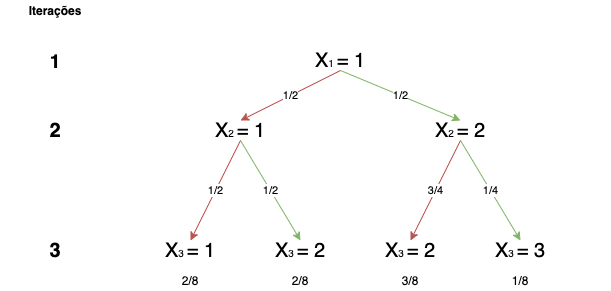
\includegraphics[scale=0.50]{figuras/morris-tree.png}
	\caption{Árvore de decisão para determinar $\Ebb\big(2^{X_3} - 1\big)$ no algoritmo \proc{Morris}. A fração próxima de 
  cada folha indica a probabilidade de $X_3$ assumir o valor em seu rótulo.}\label{fig:morris-tree}

\end{figure}

Inspecionando as folhas da árvore acima, vemos que
\begin{align*}
  \Ebb\big(2^{X_3} - 1\big) 
    &=  \frac{2}{8} \times \big(2^1 - 1\big) + \frac{2}{8} \times \big(2^2 - 1\big) + \frac{3}{8} \times 
        \big(2^2 - 1\big) + \frac{1}{8} \times \big(2^3 - 1\big) \\
    &= \frac{2}{8} \times 1 + \frac{2}{8} \times 3 + \frac{3}{8} \times 3 + \frac{1}{8} \times 7 \\
    &= \frac{24}{8} \\
    &= 3 \ .
\end{align*}

Em todos os exemplos calculados até agora, vimos que $\Ebb\big(2^{k} - 1\big) = k$. Após ganharmos intuição sobre
$\Ebb\big(2^{k} - 1\big)$ com valores pequenos de $k$, estamos preparados para demonstrar a validade da relação 
invariante.

\begin{proof}[Demonstração \ (da relação invariante)]
  A prova será por indução no número $k$ de elementos de $\Mbb$ já examinados. Vimos anteriormente que 
  $\Ebb\big(2^0 - 1 \big) = 0$ e asssim, a relação vale para $k = 0$.

  Suponhamos, agora, que a relação invariante vale para algum $k - 1$, $k \geq 1$. Mostraremos que isso implica que esta
  relação vale para $k$. Dessa forma, temos que

  \begin{align}
      \Ebb\big(2^{X_k} - 1\big) 
      &= \Ebb\big(2^{X_{k-1}}\big)  \label{proof:morris:01}  \\
      &= \Ebb\big(2^{X_{k-1}}\big) - 1 + 1 \nonumber \\
      &= \Ebb\big(2^{X_{k-1}} - 1\big) + 1 \nonumber \\
      &= k - 1 + 1 \label{proof:morris:02} \\ 
      &= k \nonumber,
    \end{align}    

    em que a igualdade~\eqref{proof:morris:01} é decorrência da identidade~\eqref{morris:rec:e} e a 
    igualdade~\eqref{proof:morris:02}, da hipótese de indução. Finalmente, a validade da relação invariante segue do 
    princípio da indução finita.
\end{proof}  

Saber que $\Ebb(\proc{Morris}(\Mbb)) = |\Mbb| = n$ não é suficiente para garantir a qualidade do estimador $2^{X} - 1$
devolvido pelo algoritmo. É desejável que além do valor esperado ser próximo ou igual ao tamnho do conjunto $\Mbb$, que
a variância da variável aleatória \proc{Morris}($\Mbb$) não seja \textit{muito grande}. Intuitivamente, isso nos diria 
que a probabilidade do estimador calculado ser longe do valor esperado é pequena. Então, apresentaremos o valor da 
variância de $\proc{Morris}(\Mbb)$ no próximo teorema.

\begin{theorem}[da variância]
  \label{morris:theorem:variance}
  Se $\Mbb$ é um conjunto com $n$ elementos, então $\Vbb(\Ebb(\morrisestimator)) = n(n - 1) / 2$.
\end{theorem}

\begin{proof}[Demonstração \ (da variância)]
  Pela definição da \hyperref[ap:variance]{variância} de uma variável aleatória, temos que

  \begin{align}
    \Vbb(\proc{Morris}(\Mbb))
    &= \Ebb(\proc{Morris}(\Mbb)^2) - \Ebb^2(\proc{Morris}(\Mbb)) \nonumber \\ 
    &= \Ebb\big(\big(2^{X_n} - 1\big)^2\big) - n^2 \label{proof:morris:var:01} \\
    &= \Ebb\big(2^{2X_n} - 2\big(2^{X_n}\big) + 1\big) - n^2 \nonumber \\
    &= \Ebb\big(2^{2X_n}\big) - 2\Ebb\big(2^{X_n}\big) + 2 - 2 + 1 - n^2 \nonumber \\
    &= \Ebb\big(2^{2X_n}\big) - 2\Ebb\big(2^{X_n} - 1\big) - 2 + 1 - n^2 \nonumber \\
    &= \Ebb\big(2^{2X_n}\big) - 2n - 1 - n^2 \label{proof:morris:var:02} \ ,
  \end{align}

  em que utilizamos a identidade $\Ebb(\proc{Morris}(\Mbb)) = \Ebb\big(2^{X_n} - 1\big) = n$ nas igualdades~
  \eqref{proof:morris:var:01}~e~\eqref{proof:morris:var:02}.

  Logo em seguida, passaremos a calcular $\Ebb\big(2^{2X_n}\big)$. Para isso, procederemos de maneira idêntica ao que 
  foi feito na demonstração do Teorema~\hyperref[morris:theorem:expected_value]{do valor esperado} utilizando a 
  recorrência~\eqref{morris:rec:xk}. Assim,

  \begin{align}
    \Ebb\big(2^{2X_n}\big)
    &=  \Ebb\Big(\Big(1 - \frac{1}{2^{X_n}}\Big) \times 2^{2X_{n - 1}} + \frac{1}{2^{X_n}} \times 2^{2(X_{n-1} 
        + 1)}\Big) \nonumber \\
    &=  \Ebb\bigg(2^{2X_{n-1}} - \frac{2^{2X_{n-1}}}{2^{X_{n-1}}} + \frac{2^{2(X_{n-1}+1)}}{2^{X_{n-1}}}\bigg) 
        \nonumber \\
    &= \Ebb\big(2^{2X_{n-1}} -2^{X_{n-1}} + 2^{X_{n-1}+2}\big) \nonumber \\
    &= \Ebb\big(2^{2X_{n-1}} + 3 \times 2^{X_{n-1}}\big) \nonumber \\
    &= \Ebb\big(2^{2X_{n-1}}\big) + 3\Ebb\big(2^{X_{n-1}}\big) \label{proof:morris:var:03} \\
    &= \Ebb\big(2^{2X_{n-1}}\big) + 3n  \ . \nonumber
  \end{align}

  A igualdade~\eqref{proof:morris:var:03} segue da identidade~\eqref{morris:rec:e}. E o valor de 
  $\Ebb\big(2^{2X_n}\big)$ pode ser obtido da expansão \textit{telescópica} da relação de recorrência

  \begin{align*}
    \Ebb\big(2^{2X_n}\big)
    &= \Ebb\big(2^{X_{n-1}}\big) + 3n \\
    &=  \Ebb\big(2^{X_{n-2}}\big) + 3(n - 1) + 3n \\
    &=  \Ebb\big(2^{X_{n-3}}\big) + 3(n - 2) + 3(n - 1) + 3n \\
    &\hspace{5mm} \vdots\\
    &=1 + 3 + \dots + 3(n-2) + 3(n-1) + 3n \\
    &=\frac{3n(n+1)}{2} + 1 \ .
  \end{align*}

  Finalmente, utilizando esse valor para prosseguir com \eqref{proof:morris:var:02}, obtemos

  \begin{align*}
    \Vbb(\proc{Morris}(\Mbb))
    &= \Ebb\big(2^{2X_n}\big) - 2n - 1 - n^2 \\
    &= \frac{3n(n+1)}{2} + 1 - 2n -1 -n^2 \\
    &= \frac{3n(n+1) - 4n - 2n^2}{2} \\
    &= \frac{n(n-1)}{2} \ .
  \end{align*}

\end{proof}

Dessa forma, podemos estimar o erro do algoritmo \proc{Morris} a partir dos Teoremas 
\hyperref[morris:theorem:expected_value]{do valor esperado} e \hyperref[morris:theorem:variance]{da variância}. Seja
$\sigma$ o desvio padrão de \proc{Morris}($\Mbb$). A \hyperref[ap:chebyshev]{desigualdade de Cherbyshev} nos diz que 
para todo $c > 0$, 
\begin{align}
  \Pbb(|\proc{Morris}(\Mbb) - n| \geq c\sigma) \leq \frac{1}{c^2} \ .  \label{morris:error}
\end{align}

Pondo $c = 4\sqrt{2}$ em \eqref{morris:error}, obtemos que 
\begin{align}
  \Pbb\big(|\proc{Morris}(\Mbb) - n| \geq 4\sqrt{2} \times \sigma\big) \leq \frac{1}{(4\sqrt{2})^2} = \frac{1}{32} \ .
\end{align}

Como pelo Teorema \hyperref[morris:theorem:variance]{da variância},
\[ \sigma^2 = \Vbb(\proc{Morris}(\Mbb)) = \frac{n(n-1)}{2} \ , \] vale que
\[ \sigma < \frac{n}{\sqrt{2}} \ . \]

Logo, temos que
\[  \Pbb\bigg(|\proc{Morris}(\Mbb) - n| \geq 4\sqrt{2} \times \frac{2}{\sqrt{2}}\bigg) =  
    \Pbb(|\proc{Morris}(\Mbb) - n| \geq 4n) \leq \frac{1}{32} \ . \]
    
Portando, podemos concluir que 
\[ \Pbb(|\proc{Morris}(\Mbb) - n| \geq 4n) \leq \frac{1}{32} < 0,032 \ . \]

Em palavras, isto nos diz que com probabilidade maior que $96,8\%$, o erro relativo cometido por \proc{Morris}($\Mbb$) é
menor do que 4.

Por fim, voltemos nossa atenção para uma das motivações iniciais do trabalho de Morris: o espaço utilizado pelo 
algoritmo. Por espaço, queremos dizer o número de bits que o algoritmo \proc{Morris} necessita para representar o 
contador~$X$ definido na linha~\ref{li:morris:init}. Denotaremos por \proc{bits}($i$) como sendo o menor número de bits
para representar um número inteiro não-negativo $i$. Temos que \proc{bits}(0) = 1 e para $i \geq 1$, \proc{bits}($i$) = 
$\lfloor\lg i\rfloor + 1$.

\begin{theorem}
  \label{morris:theorem:space}
  Sejam $\Mbb$ um conjunto com $n \geq 2$ elementos, $X$ a variável definida na linha~\ref{li:morris:init} do algoritmo
  \proc{Morris} e $b$ um número inteiro positivo. Se $X_n$ é o valor da variável~$X$ ao final de \proc{Morris}($\Mbb$), 
  então $\Pbb(\proc{bits}(X_n) \geq b + \lg\lg n + 1) \leq 1/(n^{2^b-1}-1)$.
\end{theorem}

Consideremos um exemplo para decifrar o significado do Teorema~\ref{morris:theorem:space}. Suponhamos que $\Mbb$ é um 
conjunto com $n = 2^{16} = 65536$ elementos. Neste caso, temos que $\lg \lg n = 4$. O teorema nos diz que para $b = 1$,
a representação de $X = X_{65536}$ utilizará 6 bits com probabilidade menor ou igual a 
$1/(65536^{2^1 - 1}) = 1/65536 < 1,53 \times 10^{-5}$. E para $b = 2$, seriam necessários 7 bits com probabilidade menor
ou igual a $1/(65536^{2^2 - 1}) < 3,56 \times 10^{-15}$. Nesse sentido, o Teorema~\ref{morris:theorem:space} nos garante 
que o algoritmo \proc{Morris} consome \textit{quase certamente} não mais que $\lceil\lg \lg n\rceil$ bits de espaço.

\begin{proof}[Demonstração \ (do Teorema~\ref{morris:theorem:space})]
  A \hyperref[ap:markov]{desigualdade de Markov} nos diz que para todo número real positivo $c$ vale que
  \begin{align}
    \Pbb(\proc{Morris}(\Mbb) \geq c) \leq \frac{\proc{Morris}(\Mbb)}{c} = \frac{n}{c} \ . \label{morris:markov}
  \end{align}
  Pondo $c = n^{2^b} - 1$ em \eqref{morris:markov}, obtemos que
  \begin{align}
    \Pbb\big(\proc{Morris}(\Mbb) \geq n^{2^b} - 1\big) \leq \frac{1}{n^{2^b-1} - 1} \ . \label{morris:memory:step}
  \end{align}
  Como $\proc{Morris}(\Mbb) = 2^{X_n} - 1$, reescrevendo e desenvolvendo \eqref{morris:memory:step}, encontramos que
  \begin{align*}
    \Pbb\big(2^{X_n} - 1 \geq n^{2^b} - 1\big)
    &=  \Pbb\big(2^{X_n} \geq n^{2^b}\big) \\
    &=  \Pbb\big(X_n \geq \lg n^{2^b}\big) \\
    &=  \Pbb\big(\lg X_n \geq \lg \lg n^{2^b}\big) \\
    &\geq  \Pbb\big(\lfloor\lg X_n\rfloor \geq \lg \lg n^{2^b}\big) \\
    &=  \Pbb\big(\lfloor\lg X_n\rfloor + 1 \geq \lg \lg n^{2^b} + 1\big) \\
    &=  \Pbb\big(\proc{bits}(X_n) \geq \lg \lg n^{2^b} + 1\big) \\
    &=  \Pbb\big(\proc{bits}(X_n) \geq \lg 2^{b} + \lg \lg n + 1\big) \\
    &=  \Pbb(\proc{bits}(X_n) \geq b + \lg \lg n + 1) \ .
  \end{align*}
  Combinando a desigualdade acima com \eqref{morris:memory:step}, vemos que
  \[  \Pbb(\proc{bits}(X_n) \geq b + \lg \lg n + 1) \leq \frac{1}{n^{2^b-1} - 1} \ . \]
  Com isto, concluímos a prova do teorema.
\end{proof}

\section{\proc{Morris} e a lei dos grandes números}
\label{sec:morris:plus}

Pela análise \ref{sec:morris:analysis} do Algoritmo \ref{prog:morris}, nota-se que esta solução apresenta uma grande variabilidade. 
Esta seção busca abordar uma técnica para diminuir este problema e, também, é baseada nas notas de aula de \citep{LectureNotesAndoni}.

A ideia principal é executar $k$ vezes o Algoritmo \ref{prog:morris} e a nova estimativa será a média aritmética dos resultados
de cada execução. Será visto que isso diminuirá a variância da estimativa.

Segue o pseudocódigo do algoritmo adaptado:
\begin{programruledcaption}{
Algoritmo de Morris adaptado\label{prog:morris:plus}
\\ \textbf{Entrada:} conjunto $\Mbb$, quantidade $K$ de iterações do Algoritmo \ref{prog:morris} 
\\ \textbf{Saída:} estimativa de $|\Mbb|$
\label{prog:flajolet-martin}
}
  \begin{lstlisting}[
    language={[brazilian]pseudocode},
    style=pseudocode,
    style=wider,
    functions={},
    specialidentifiers={},
    deletekeywords={de}
  ]
      função Morris++($\Mbb$, $K$)
        Y := 0
        para k de 1 até K \kw{faça}
          $\tilde{X}_k$ := Morris($\Mbb$)
          Y := Y + $\tilde{X}_k$
        fim
        devolva $\frac{Y}{K}$
      fim
  \end{lstlisting}
\end{programruledcaption}

Considere que $Y_n$ é a saída do Algoritmo \ref{prog:morris:plus} para uma entrada de tamanho $n$.

\begin{lemma}\label{morris:plus:expected_value}
  $\Ebb[Y_n] = n$.
\end{lemma}

\begin{proof}

\begin{align*}
  \Ebb[Y_n] 
    &= \Ebb \Big[ \frac{1}{k} \sum_{i=1}^{k} X_n \Big]  \\
    &= \frac{1}{k} \sum_{i=1}^{k} \Ebb[X_n] \\
    &= \frac{1}{k} k n  \\
    &= n \ .
\end{align*}

\end{proof}

\begin{lemma}\label{morris:plus:variance}
  $\Vbb[Y_n] \leq \frac{1}{k} ( \frac{3n(n+1)}{2} + 1 )$.
\end{lemma}

\begin{proof}
  
\begin{align*}
  \Vbb[Y_n] 
    &= \Vbb[\frac{1}{k} \sum_{i=1}^{k} X_n] \\
    &= \frac{1}{k^2} \sum_{i=1}^{k}\Vbb[X_n]  \\
    &\leq \frac{1}{k^2} \sum_{i=1}^{k} \Big( \frac{3n(n+1)}{2} + 1 \Big)  \\
    &= \frac{1}{k^2} k \Big( \frac{3n(n+1)}{2} + 1 \Big)  \\
    &= \frac{1}{k} \Big( \frac{3n(n+1)}{2} + 1 \Big) \ .
\end{align*}

\end{proof}

Agora, pode-se usar os Lemas \ref{morris:plus:expected_value} e \ref{morris:plus:variance} para se conseguir uma estimativa para o 
erro do Algoritmo \ref{prog:morris:plus}. De forma análoga ao que foi feito na conclusão da Análise \ref{sec:morris:analysis}, pode-se 
concluir que

\[ \mathbb{P}(|Y_n - n| \geq \epsilon n ) \leq \frac{2}{\epsilon^2 k} \ . \]

em que $\epsilon$ é o erro relativo do Algoritmo \ref{prog:morris:plus} e $k$, a quantidade de execuções do Algoritmo \ref{prog:morris}.
Assim, para um intervalo de confiança de $\delta$, pode-se escrever $k$ em função de $\epsilon$ e $\delta$:

\begin{align*}
      &\frac{2}{\epsilon^2 k^2} = 1 - \delta \\
  \iff& k = \Bigg\lceil \frac{2}{(1 - \delta) \epsilon^2} \Bigg\rceil \ .
\end{align*}

Por fim, fixando um intervalo de confiança de $95\%$ e erro relativo de $10\%$ ($\epsilon = 0.1$), $k$ deve ser $4000$.  
